\documentclass[aspectratio=169,11pt]{beamer}
\usepackage[T1]{fontenc}
\usepackage{lmodern,amsmath,amssymb,mathtools,bm,booktabs,array,graphicx,tikz}
\usetikzlibrary{arrows.meta,positioning,calc,decorations.pathreplacing,patterns}
\definecolor{ink}{HTML}{17344D}\definecolor{accent}{HTML}{087E8B}\definecolor{pale}{HTML}{EDF5F5}\definecolor{gold}{HTML}{AD6B19}
\providecommand{\dd}{\,\mathrm{d}}\providecommand{\R}{\mathbb{R}}
\providecommand{\E}{\mathbb{E}}\providecommand{\Var}{\operatorname{Var}}
\providecommand{\Cov}{\operatorname{Cov}}\providecommand{\diag}{\operatorname{diag}}
\providecommand{\norm}[1]{\left\lVert#1\right\rVert}
\providecommand{\abs}[1]{\left|#1\right|}
\usefonttheme{professionalfonts}
\setbeamercolor{normal text}{fg=black,bg=white}
\setbeamercolor{frametitle}{fg=ink,bg=white}
\setbeamercolor{title}{fg=ink}\setbeamercolor{structure}{fg=accent}
\setbeamercolor{block title}{fg=ink,bg=pale}\setbeamercolor{block body}{fg=black,bg=pale!40}
\setbeamercolor{alerted text}{fg=accent}
\setbeamerfont{frametitle}{size=\Large,series=\bfseries}
\setbeamerfont{title}{size=\LARGE,series=\bfseries}
\setbeamertemplate{navigation symbols}{}
\setbeamersize{text margin left=.7cm,text margin right=.7cm}
\setbeamertemplate{frametitle}{\vspace{.18cm}\insertframetitle\par\vspace{.1cm}{\color{accent}\hrule height .6pt}\vspace{.12cm}}
\newcommand{\notestarget}{notes.pdf}\newcommand{\noteslabel}{Notes}
\setbeamertemplate{footline}{\hspace{.7cm}\color{ink}\scriptsize Mathematical Cardiology\quad\href{\notestarget}{\noteslabel}\hfill\insertframenumber\,/\,\inserttotalframenumber\hspace{.7cm}\vspace{.18cm}}
\setbeamercovered{invisible}
\hypersetup{pdfauthor={Zan Ahmad},pdftitle={The circulation},pdfpagemode=UseNone}
\begin{document}
\begin{frame}[plain]\vfill
{\small\color{accent} Mathematical Cardiology \quad Lecture 1}\par\medskip
{\raggedright\hyphenpenalty=10000\exhyphenpenalty=10000\LARGE\bfseries\color{ink} The circulation}\par\bigskip
Zan Ahmad\par\smallskip
{\small Fall 2023}\par\vfill\end{frame}
\renewcommand{\notestarget}{notes.pdf\#note-the-route-and-the-direction-convention}
\begin{frame}[t,fragile,label=slide-the-circulation-as-a-closed-route]{The circulation as a closed route}
\[\begin{gathered}\text{left heart}\to\text{systemic bed}\to\text{right heart},\\\text{right heart}\to\text{pulmonary bed}\to\text{left heart}.\end{gathered}\]\pause{} A route specifies connections. It does not yet determine the flow on any connection.
\end{frame}
\renewcommand{\notestarget}{notes.pdf\#note-the-route-and-the-direction-convention}
\begin{frame}[label=slide-chambers-valves-and-vascular-beds-figure]{Chambers, valves, and vascular beds}
\centering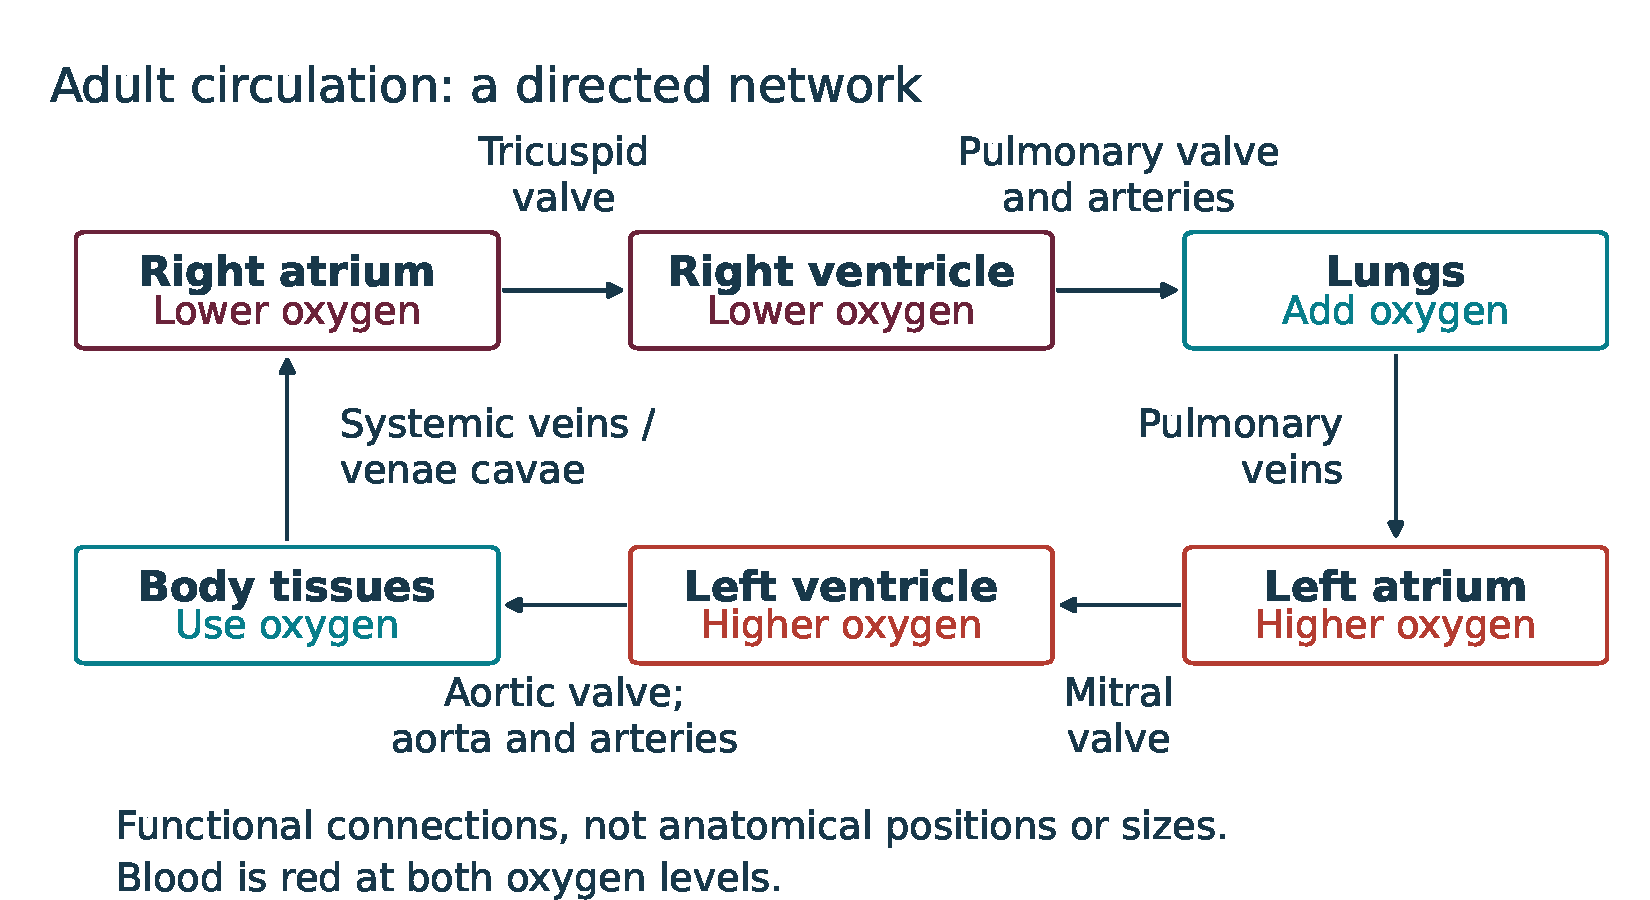
\includegraphics[width=.98\linewidth,height=.69\textheight,keepaspectratio]{presentation-figures/network-slide.pdf}\end{frame}
\renewcommand{\notestarget}{notes.pdf\#note-the-route-and-the-direction-convention}
\begin{frame}[t,fragile,label=slide-chambers-valves-and-vascular-beds]{Chambers, valves, and vascular beds}
The pulmonary and systemic beds are in series.\pause{}\par Within a bed, individual vessels branch and rejoin.\pause{}\par Arteries and veins are named by direction relative to the heart, not by oxygen content.
\end{frame}
\renewcommand{\notestarget}{notes.pdf\#note-an-amount-and-a-rate-are-different-variables}
\begin{frame}[t,fragile,label=slide-choose-the-quantity]{Choose the quantity}
\begin{center}\begin{tabular}{lll}\toprule Variable & Meaning & Unit\\\midrule $V$ & stored volume & L\\ $Q$ & volume per time & L/min\\ $P$ & pressure & mmHg\\\bottomrule\end{tabular}\end{center}\pause{} A numerical value without its unit does not identify the quantity.
\end{frame}
\renewcommand{\notestarget}{notes.pdf\#note-an-amount-and-a-rate-are-different-variables}
\begin{frame}[t,fragile,label=slide-from-a-rate-to-a-passing-volume]{From a rate to a passing volume}
\[\Delta V_{\rm passed}=Q\Delta t\]\pause{}\[\left(5\frac{\mathrm L}{\mathrm{min}}\right)\left(\frac{30}{60}\mathrm{min}\right)=2.5\mathrm L.\]\pause{} This is not the net increase of volume inside the body.
\end{frame}
\renewcommand{\notestarget}{notes.pdf\#note-an-amount-and-a-rate-are-different-variables}
\begin{frame}[t,fragile,label=slide-average-output-per-minute]{Average output per minute}
\[Q=FV_s\]\pause{}\[\frac{\mathrm{beats}}{\mathrm{min}}\frac{\mathrm L}{\mathrm{beat}}=\frac{\mathrm L}{\mathrm{min}}.\]\pause{} A change in $F$ does not specify the change in $FV_s$ unless the change in $V_s$ is also known.
\end{frame}
\renewcommand{\notestarget}{notes.pdf\#note-pressure-enters-through-a-difference}
\begin{frame}[t,fragile,label=slide-the-pressure-drop]{The pressure drop}
\[\Delta P=P_{\rm in}-P_{\rm out}\]\pause{}\[95-5=90\ \mathrm{mmHg},\qquad95-50=45\ \mathrm{mmHg}.\]\pause{} The same inlet pressure can accompany different driving differences.
\end{frame}
\renewcommand{\notestarget}{notes.pdf\#note-pressure-enters-through-a-difference}
\begin{frame}[t,fragile,label=slide-a-reference-shift-cancels]{A reference shift cancels}
\[\Delta P_{\rm new}=(P_{\rm in}+P_0)-(P_{\rm out}+P_0).\]\pause{}\[\Delta P_{\rm new}=P_{\rm in}-P_{\rm out}.\]\pause{} Changing the reference is different from physically changing the surrounding pressure of a flexible vessel.
\end{frame}
\renewcommand{\notestarget}{notes.pdf\#note-a-resistance-is-a-physical-assumption}
\begin{frame}[t,fragile,label=slide-the-linear-resistance-law]{The linear resistance law}
\[\Delta P=RQ,\qquad R>0.\]\pause{}\[Q=\frac{\Delta P}{R},\qquad[R]=\frac{\mathrm{mmHg}}{\mathrm{L/min}}.\]\pause{} Assumptions: prescribed pressures, fixed resistance, and negligible storage within this element.
\end{frame}
\renewcommand{\notestarget}{notes.pdf\#note-a-resistance-is-a-physical-assumption}
\begin{frame}[label=slide-one-controlled-resistance-comparison-figure]{One controlled resistance comparison}
\centering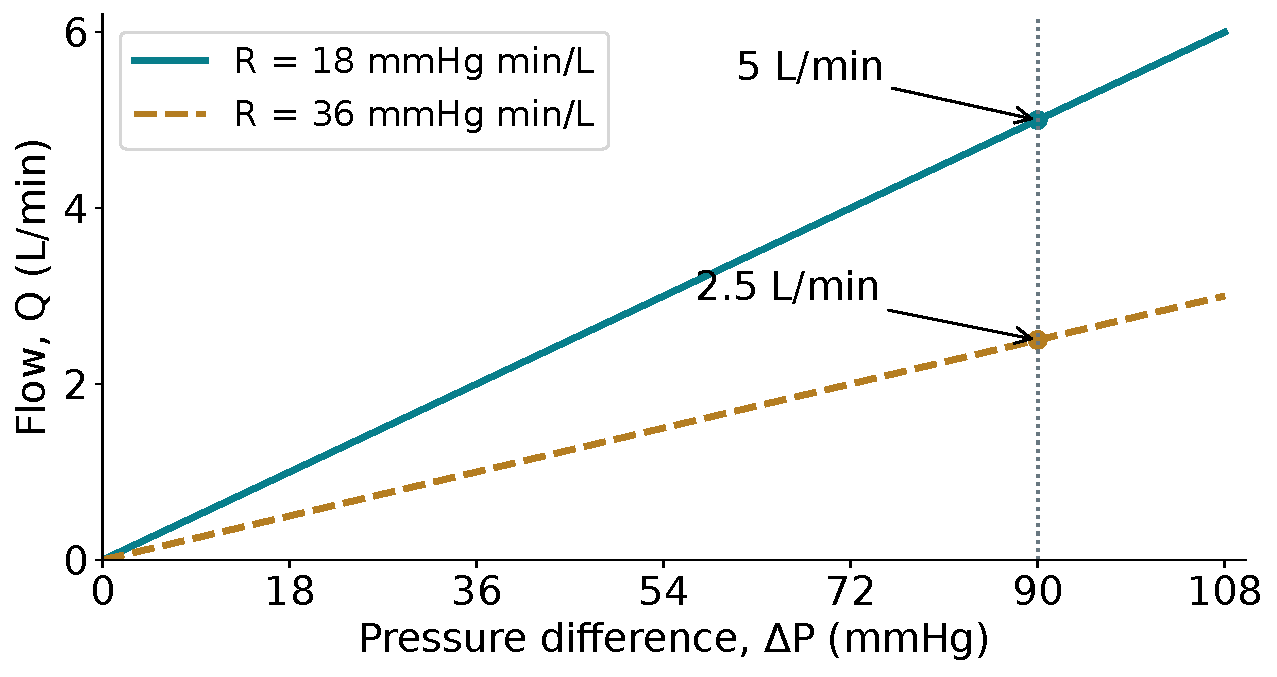
\includegraphics[width=.98\linewidth,height=.69\textheight,keepaspectratio]{presentation-figures/pressure-flow.pdf}\end{frame}
\renewcommand{\notestarget}{notes.pdf\#note-a-resistance-is-a-physical-assumption}
\begin{frame}[t,fragile,label=slide-one-controlled-resistance-comparison]{One controlled resistance comparison}
\[Q_1=\frac{95-5}{18}=5\ \mathrm{L/min}.\]\pause{}\[Q_2=\frac{95-5}{36}=2.5\ \mathrm{L/min}.\]\pause{} Only resistance changed. A whole-circulation response need not preserve the same pressure drop.
\end{frame}
\renewcommand{\notestarget}{notes.pdf\#note-a-resistance-is-a-physical-assumption}
\begin{frame}[t,fragile,label=slide-fixed-pressure-and-fixed-flow]{Fixed pressure and fixed flow}
\[\frac{Q_2}{Q_1}=\frac{\Delta P_2}{\Delta P_1}\frac{R_1}{R_2}.\]\pause{} If $\Delta P_2=\Delta P_1$, doubling $R$ halves $Q$.\pause{}\par If $Q_2=Q_1$, doubling $R$ requires twice the pressure difference.
\end{frame}
\renewcommand{\notestarget}{notes.pdf\#note-a-resistance-is-a-physical-assumption}
\begin{frame}[t,fragile,label=slide-sign-and-limiting-cases]{Sign and limiting cases}
\[\Delta P=0\Rightarrow Q=0.\]\pause{}\[\Delta P<0\Rightarrow Q<0\quad(R>0).\]\pause{} A one-way valve requires an extra rule; a signed resistance alone does not enforce one-way flow.
\end{frame}
\renewcommand{\notestarget}{notes.pdf\#note-conservation-begins-with-a-chosen-boundary}
\begin{frame}[t,fragile,label=slide-count-volume-crossing-a-boundary]{Count volume crossing a boundary}
\[\Delta V=\Delta t\left(\sum Q_{\rm in}-\sum Q_{\rm out}\right).\]\pause{} A positive balance increases storage.\pause{}\par A zero balance is a statement about the sum of the connections.
\end{frame}
\renewcommand{\notestarget}{notes.pdf\#note-conservation-begins-with-a-chosen-boundary}
\begin{frame}[t,fragile,label=slide-a-branch-does-not-duplicate-flow]{A branch does not duplicate flow}
\[Q_0=Q_1+Q_2\qquad\text{when storage does not change}.\]\pause{} For example, $5=2+3$ L/min.\pause{}\par Each branch can carry a different flow while the junction conserves volume.
\end{frame}
\renewcommand{\notestarget}{notes.pdf\#note-conservation-begins-with-a-chosen-boundary}
\begin{frame}[t,fragile,label=slide-internal-transfers-cancel]{Internal transfers cancel}
\begin{align*}\Delta V_1&=(Q_{\rm in}-q)\Delta t,\\\Delta V_2&=(q-Q_{\rm out})\Delta t.\end{align*}\pause{}\[\Delta(V_1+V_2)=(Q_{\rm in}-Q_{\rm out})\Delta t.\]
\end{frame}
\renewcommand{\notestarget}{notes.pdf\#note-conservation-begins-with-a-chosen-boundary}
\begin{frame}[t,fragile,label=slide-instantaneous-flow-and-cycle-average]{Instantaneous flow and cycle average}
A chamber may store blood during part of a beat.\pause{}\par If its volume returns to its starting value after one complete cycle,\[\text{volume entering per cycle}=\text{volume leaving per cycle}.\]\pause{} This is an average constraint, not equality at every instant.
\end{frame}
\renewcommand{\notestarget}{notes.pdf\#note-pressure-rise-supplied-by-the-pump}
\begin{frame}[t,fragile,label=slide-why-the-loop-needs-a-pump]{Why the loop needs a pump}
\[\Delta P_{\rm pump}-R_1Q-\cdots-R_mQ=0.\]\pause{}\[\Delta P_{\rm pump}=Q\sum_iR_i.\]\pause{} With no pressure rise and positive resistances, the steady series model gives $Q=0$.
\end{frame}
\renewcommand{\notestarget}{notes.pdf\#note-pressure-rise-supplied-by-the-pump}
\begin{frame}[t,fragile,label=slide-from-one-element-to-a-circulation]{From one element to a circulation}
The resistance calculation determines $Q$ from prescribed pressures.\pause{}\par A closed circulation must also determine those pressures from pumping, storage, and conservation.\pause{}\par The next construction adds an elastic reservoir.
\end{frame}
\end{document}
